\section{Regra do Trapézio}

\begin{figure}[htb]
 \centering
\begin{minipage}[c]{7cm}
    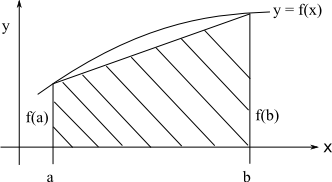
\includegraphics[scale=0.8]{capitulos/capitulo2/figuras/regra_trapezio1.png}
    \caption{Área sob a reta representando a integral}
    \label{fig:regra_trapezio1}
 \end{minipage}\hspace*{1cm}
 \begin{minipage}[c]{6cm}
    \begin{equation}
     \label{cap2:sec2:eq1}
     I = \int_a^b \, f\,(x) \, dx = \frac{b - a}{2} \, [f\,(a) + f\,(b)] + E
    \end{equation}

    onde \esp{E = \mbox{erro}}.
 \end{minipage}
\end{figure}

\subsection{Erro da Regra do Trapézio}

\[
 E = \int_a^b \, f\,(x) \, dx - \frac{b - a}{2} \, [f\,(a) + f\,(b)]
\]

Expansão de Taylor de \esp{f(x)} na vizinhança de \esp{\overline{x} = \frac{a + b}{2}}

\[
 f\,(x) = f\,(\overline{x}) + \frac{f'(\overline{x})}{1!} \, (x - \overline{x}) + \frac{f''(\overline{x})}{2!} \, (x - \overline{x})^2 + \ldots
\]

Assim,

\begin{equation}
 \label{cap2:sec2:eqA}
 \begin{array}{ll}
  \displaystyle \int_a^b f\,(x) \, dx & = f\,(\overline{x}) \left. \, x \, \right|_a^b + f'(\overline{x}) \, \left\{ \left. \displaystyle \frac{x^2}{2} \, \right|_a^b - \overline{x} \left. \, x \, \right|_a^b \right\} + \displaystyle \frac{f''(\overline{x})}{2} \left\{ \left. \frac{x^3}{3} \, \right|_a^b - \overline{x} \left. \, x^2 \, \right|_a^b \, \overline{x}^{\,2} \left. \, x \, \right|_a^b \right\} \\
                        & = f\,(\overline{x}) \, (b - a) + f'(\overline{x}) \, \left\{ \displaystyle \frac{(b - a)}{1} \, \underbrace{\frac{(b + a)}{2}}_{\overline{x}} - \overline{x} \, (b - a) \right\} + \\
                        & + \displaystyle \frac{f''(\overline{x})}{2} \, \left\{ \frac{b^3 - a^3}{3} - \overline{x} \, (b^2 - a^2) + \overline{x}^{\,2} \, (b - a) \right\} \\
                        & = f\,(\overline{x}) \, (b - a) + \displaystyle \frac{1}{24} \, f''(\overline{x}) \, (b - a)^3 + \ldots
 \end{array}
\end{equation}

\begin{equation}
 \label{cap2:sec2:eqB}
 \begin{array}{ll}
  \displaystyle \frac{b - a}{2} \, [f\,(a) + f\,(b)] & = \displaystyle \frac{b - a}{2} \, \left\{ f\,(\overline{x}) + f'(\overline{x}) \left[ \underbrace{a - \frac{a + b}{2}}_{-\frac{1}{2}\,(b - a)} \right] + \frac{1}{2}\,f''(\overline{x}) \left[ \underbrace{a - \frac{a + b}{2}}_{-\frac{1}{2}\,(b - a)} \right]^2 + \ldots \right. \\
  \\
  & \left. + f\,(\overline{x}) + f'(\overline{x}) \, \left[ \underbrace{b - \frac{a + b}{2}}_{\frac{1}{2} \, (b - a)} \right] + \frac{1}{2} \, f''(\overline{x}) \, \left[ \underbrace{b - \frac{a + b}{2}}_{\frac{1}{2} \, (b - a)} \right]^2 \, \right\} \\
  \\
  & = \displaystyle \frac{b - a}{2} \, \left\{ 2\,f\,(\overline{x}) + f''(\overline{x}) \, \frac{1}{4} \, (b - a)^2 + \ldots \right\} \\
  & = f\,(\overline{x}) \, (b - a) + \displaystyle \frac{1}{8} \, f''(\overline{x}) \, (b - a)^3 + \ldots
 \end{array}
\end{equation}

\[
 \begin{array}{ll}
  & E \approx f''(\overline{x}) \, (b - a)^3 \, \left(\displaystyle \frac{1}{24} - \frac{1}{8}\right) \approx - \displaystyle \frac{1}{12} \, f''(\overline{x}) \, (b - a)^3 \\
  \\
  (\ref{cap2:sec2:eqA}) & \mbox{ \framebox{ $ E \approx - \displaystyle \frac{1}{12} \, f''(\overline{x}) \, h^3 $ } }
 \end{array}
\]

Se \esp{h = \displaystyle \frac{b - a}{N}}, então

\[
 \begin{array}{ll}
  (\ref{cap2:sec2:eqB}) & \mbox{ \framebox{ $ E \approx - \displaystyle \frac{1}{12} \, \frac{(b - a)^3}{N^3} \, \sum_{i=1}^N \, f''(\overline{x}_i) $ } } \\
  \\
  & \mbox{ \framebox{ $ E \approx - \displaystyle \frac{1}{12} \, (b - a) \, h^2 \, \overline{f}\,'' $ } }
 \end{array}
\]

onde

\[
 \overline{f}\,'' = \sum_{i=1}^N \, \frac{f''(\overline{x}_i)}{N}
\]

\subsection{Múltiplos Intervalos}

\begin{itemize}
 \item $n$ = número de intervalos = número de trapézios
\item $h$ = altura dos trapézios = \esp{\displaystyle \frac{b - a}{n}}
\end{itemize}

\begin{figure}[htb]
 \centering
 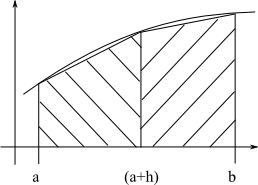
\includegraphics[scale=0.8]{capitulos/capitulo2/figuras/regra_trapezio2.png}
 \caption{Área sob a reta representando a integral com intervalos}
 \label{fig:regra_trapezio2}
\end{figure}

Suponha:

\[
 \begin{array}{ll}
  n = 2 \Rightarrow I & = \displaystyle \frac{1}{2} \left[ f\,(a) + f\,(a + h) \right] \, h + \frac{1}{2} \left[ f\,(a + h) + f\,(b) \right] \, h \vspace*{0.2cm} \\
                      & = \displaystyle \frac{h}{2} \, \left[ f\,(a) + 2\,f\,(a + h) + f\,(b) \right] \\
  \\
  n = 3 \Rightarrow I & = \displaystyle \frac{1}{2} \left[ f\,(a) + f\,(a + h) \right] \, h + \frac{1}{2} \left[ f\,(a + h) + f\,(a + 2\,h) \right] \, h + \frac{1}{2} \, \left[ f\,(a + 2\,h) + f\,(b) \right] \, h \vspace*{0.2cm} \\
                      & = \displaystyle \frac{h}{2} \, \left\{ f\,(a) + 2\,\left[ f\,(a + h) + f\,(a + 2\,h) + f\,(a + 3\,h) \right] + f\,(b) \right\} \\
  \\
  n = 4 \Rightarrow I & = \displaystyle \frac{h}{2} \left\{ f\,(a) + 2\,\left[ f\,(a + h) + f\,(a + 2\,h) + f\,(a + 3\,h) \right] + f\,(b) \right\}
 \end{array}
\]

\begin{equation}
 \begin{array}{l}
  n = N \Rightarrow \mbox{ \framebox{ $ I = \displaystyle \frac{h}{2} \left\{ f\,(a) + 2\,\sum_{i=1}^{N-1} \, f\,(a + i\,h) + f\,(b) \right\} $ } }
 \end{array}
\end{equation}

\begin{example}

\begin{figure}[htb]
 \centering
 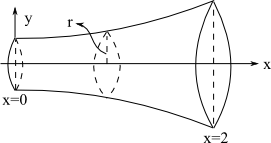
\includegraphics[scale=1.0]{capitulos/capitulo2/figuras/regra_trapezio3.png}
 \caption{Volume de superfície curva}
 \label{fig:regra_trapezio2}
\end{figure}

\[
 \overline{f}\,(x) = 1 + \left( \frac{x}{2} \right)^2, \, \, 0 \leq x \leq 2
\]

Calcule o volume

\[
 \begin{array}{ll}
  V & = \displaystyle \int_0^2 \pi \, r^2 \, dx = \int_0^2 \pi \, \left[ 1 + \frac{x^2}{4} \right]^2 \, dx = \int_0^2 \pi \, \left( 1 + \frac{x^2}{2} + \frac{x^4}{16} \right) \, dx \\
    & = \left. \pi \, \left[ x + \displaystyle \frac{x^3}{6} + \frac{x^5}{80} \right] \displaystyle \, \right|_0^2 = \pi \, \left(2 + \displaystyle \frac{2^3}{6} + \frac{2^5}{80}\right) = 11.7286
 \end{array}
\]

\end{example}